
\documentclass[a4paper,11pt]{article}
\usepackage[margin=2.5cm]{geometry}
\usepackage{hyperref}
\usepackage{longtable}
\usepackage{enumitem}
\usepackage{graphicx}
\usepackage{float}
\usepackage{tikz}
\usetikzlibrary{arrows.meta,positioning,shapes.geometric,shapes.misc,trees}
\usepackage{titlesec}
\usepackage{lmodern}
\renewcommand{\familydefault}{\sfdefault}

\title{FATE Report 2026 \\ Technical Flow Documentation }
\author{Consorzio LaMMA}
\date{\today}

\usepackage{pdflscape}

\begin{document}

\maketitle
\tableofcontents
\newpage

\section{High-Level Operational Overview}

The following diagram summarizes the production workflow from environment configuration
to final report generation. It represents the logical sequence executed during a standard
monthly production run.

\begin{figure}[H]
\centering
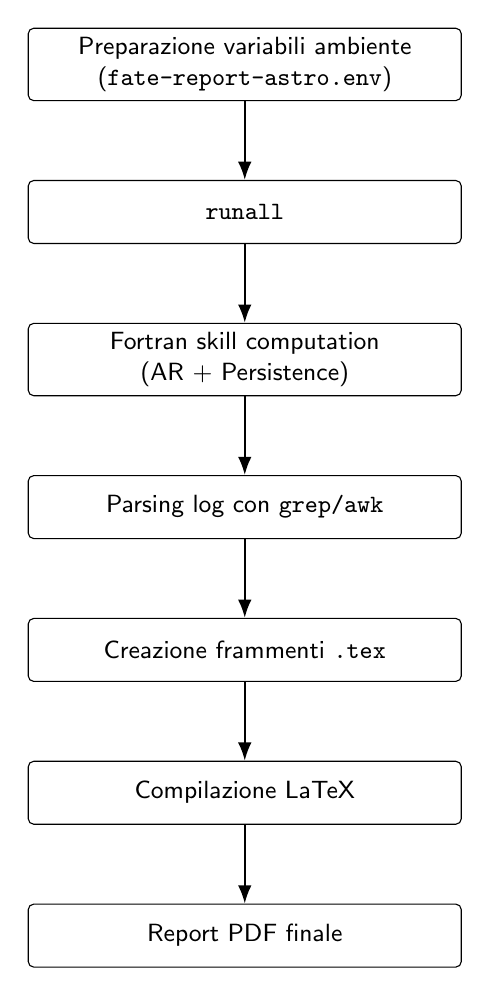
\begin{tikzpicture}[
    node distance=10mm,
    every node/.style={font=\small},
    block/.style={rectangle, draw, rounded corners=2pt, align=center, minimum width=55mm, minimum height=8mm},
    arrow/.style={-Latex, thick}
]

\node[block] (env) {Preparazione variabili ambiente \\ (\texttt{fate-report-astro.env})};
\node[block, below=of env] (runall) {\texttt{runall}};
\node[block, below=of runall] (fortran) {Fortran skill computation \\ (AR + Persistence)};
\node[block, below=of fortran] (parsing) {Parsing log con \texttt{grep/awk}};
\node[block, below=of parsing] (texgen) {Creazione frammenti \texttt{.tex}};
\node[block, below=of texgen] (latex) {Compilazione LaTeX};
\node[block, below=of latex] (pdf) {Report PDF finale};

\draw[arrow] (env) -- (runall);
\draw[arrow] (runall) -- (fortran);
\draw[arrow] (fortran) -- (parsing);
\draw[arrow] (parsing) -- (texgen);
\draw[arrow] (texgen) -- (latex);
\draw[arrow] (latex) -- (pdf);

\end{tikzpicture}
\caption{High-level operational workflow of the FATE reporting pipeline.}
\end{figure}

This diagram abstracts from implementation details and highlights the sequential
nature of the processing chain. Each block corresponds to a well-defined operational
stage with specific input/output artifacts.


\section{Overview}

\begin{itemize}
    \item The technical execution flow of \texttt{SCRIPTS/runall}
    \item The interaction between shell scripts and Fortran programs
    \item The parameters configurable in \texttt{fate-report-astro.env}
    \item The impact of each parameter on the operational pipeline
\end{itemize}

\section{High-Level Execution Flow}

\begin{figure}[H]
\centering
\resizebox{\textwidth}{!}{%
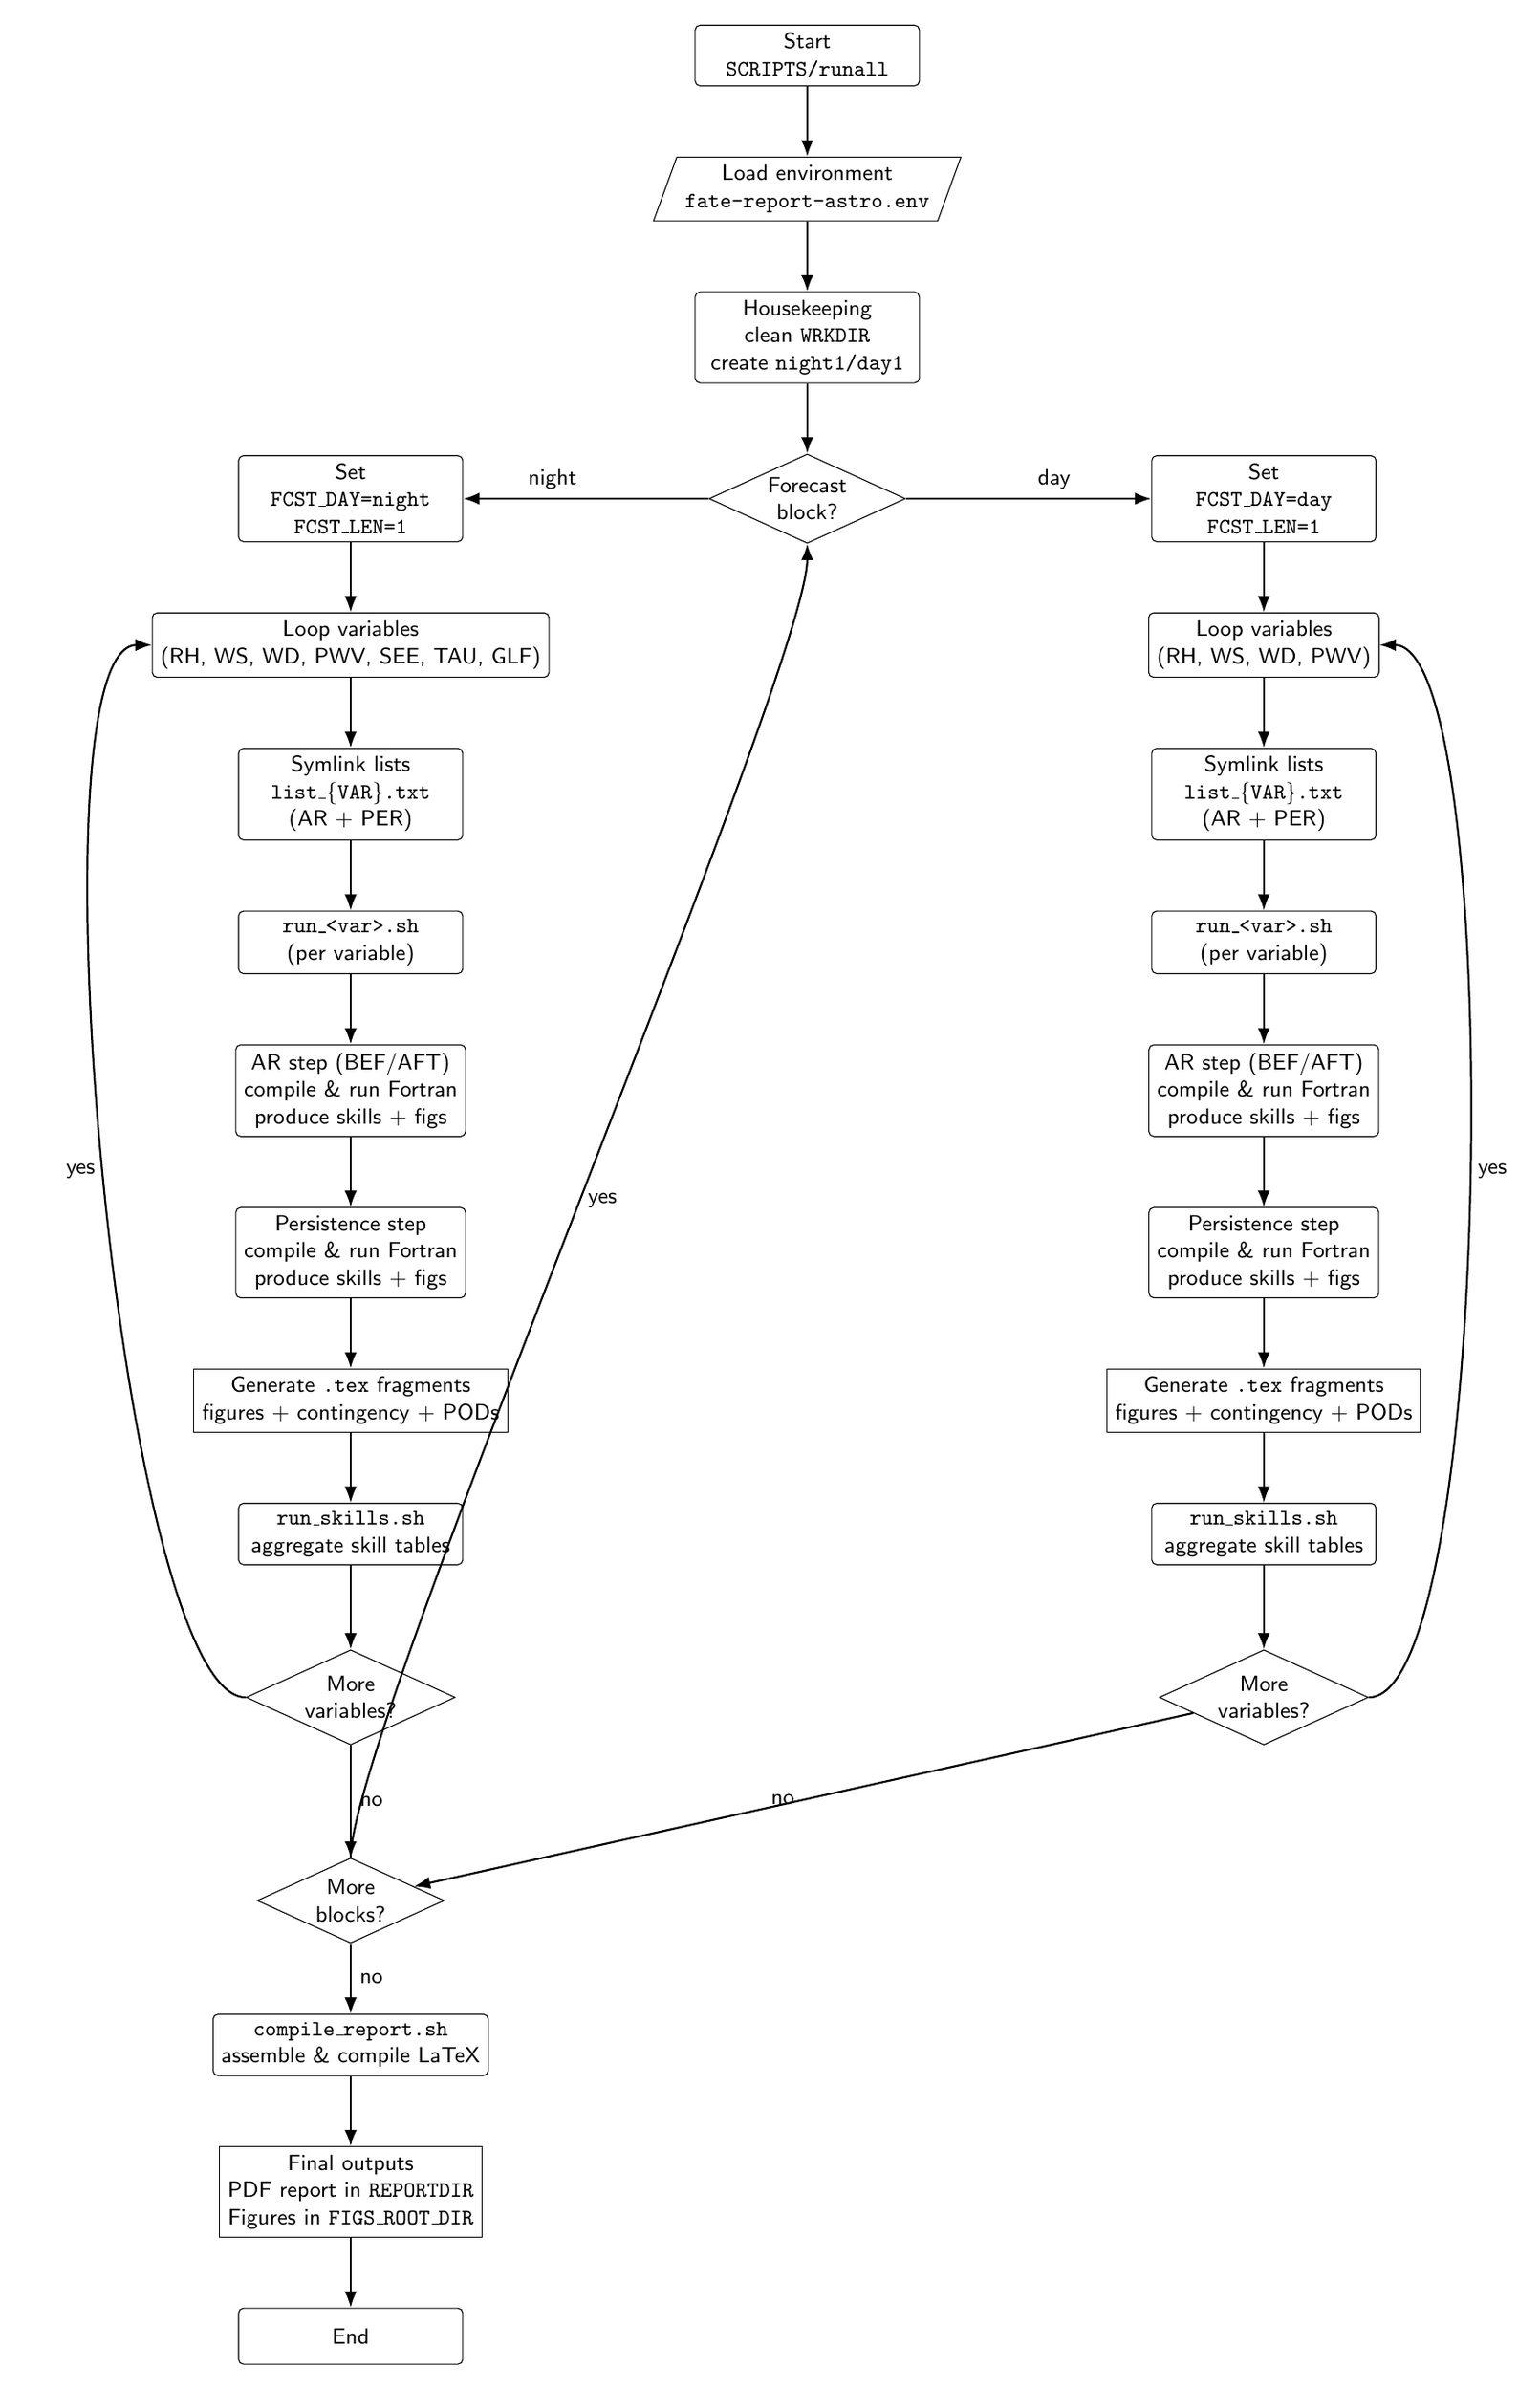
\begin{tikzpicture}[
  node distance=10mm and 10mm,
  every node/.style={font=\small},
  proc/.style={rectangle, rounded corners=2pt, draw, align=center, minimum width=32mm, minimum height=8mm},
  io/.style={trapezium, trapezium left angle=70, trapezium right angle=110, draw, align=center, minimum width=36mm, minimum height=8mm},
  doc/.style={rectangle, draw, align=center, minimum width=34mm, minimum height=8mm},
  decision/.style={diamond, draw, align=center, aspect=2.2, inner sep=1.5pt},
  arrow/.style={-Latex, thick}
]

\node[proc] (start) {Start\\\texttt{SCRIPTS/runall}};
\node[io, below=of start] (env) {Load environment\\\texttt{fate-report-astro.env}};
\node[proc, below=of env] (hk) {Housekeeping\\clean \texttt{WRKDIR}\\create \texttt{night1/day1}};
\node[decision, below=of hk] (block) {Forecast\\block?};

\node[proc, left=35mm of block] (night) {Set\\\texttt{FCST\_DAY=night}\\\texttt{FCST\_LEN=1}};
\node[proc, right=35mm of block] (day) {Set\\\texttt{FCST\_DAY=day}\\\texttt{FCST\_LEN=1}};

\node[proc, below=of night] (varloopN) {Loop variables\\(RH, WS, WD, PWV, SEE, TAU, GLF)};
\node[proc, below=of day] (varloopD) {Loop variables\\(RH, WS, WD, PWV)};

\node[proc, below=of varloopN] (symlinkN) {Symlink lists\\\texttt{list\_\{VAR\}.txt}\\(AR + PER)};
\node[proc, below=of varloopD] (symlinkD) {Symlink lists\\\texttt{list\_\{VAR\}.txt}\\(AR + PER)};

\node[proc, below=of symlinkN] (runvarN) {\texttt{run\_<var>.sh}\\(per variable)};
\node[proc, below=of symlinkD] (runvarD) {\texttt{run\_<var>.sh}\\(per variable)};

\node[proc, below=of runvarN] (arstepN) {AR step (BEF/AFT)\\compile \& run Fortran\\produce skills + figs};
\node[proc, below=of runvarD] (arstepD) {AR step (BEF/AFT)\\compile \& run Fortran\\produce skills + figs};

\node[proc, below=of arstepN] (perstepN) {Persistence step\\compile \& run Fortran\\produce skills + figs};
\node[proc, below=of arstepD] (perstepD) {Persistence step\\compile \& run Fortran\\produce skills + figs};

\node[doc, below=of perstepN] (texfragN) {Generate \texttt{.tex} fragments\\figures + contingency + PODs};
\node[doc, below=of perstepD] (texfragD) {Generate \texttt{.tex} fragments\\figures + contingency + PODs};

\node[proc, below=of texfragN] (skillsN) {\texttt{run\_skills.sh}\\aggregate skill tables};
\node[proc, below=of texfragD] (skillsD) {\texttt{run\_skills.sh}\\aggregate skill tables};

\node[decision, below=12mm of skillsN] (morevarsN) {More\\variables?};
\node[decision, below=12mm of skillsD] (morevarsD) {More\\variables?};

\node[decision, below=16mm of morevarsN] (moreblocks) {More\\blocks?};

\node[proc, below=of moreblocks] (compile) {\texttt{compile\_report.sh}\\assemble \& compile LaTeX};
\node[doc, below=of compile] (pdf) {Final outputs\\PDF report in \texttt{REPORTDIR}\\Figures in \texttt{FIGS\_ROOT\_DIR}};
\node[proc, below=of pdf] (end) {End};

% Arrows
\draw[arrow] (start) -- (env);
\draw[arrow] (env) -- (hk);
\draw[arrow] (hk) -- (block);

\draw[arrow] (block) -- node[above left]{night} (night);
\draw[arrow] (block) -- node[above right]{day} (day);

\draw[arrow] (night) -- (varloopN);
\draw[arrow] (day) -- (varloopD);

\draw[arrow] (varloopN) -- (symlinkN);
\draw[arrow] (varloopD) -- (symlinkD);

\draw[arrow] (symlinkN) -- (runvarN);
\draw[arrow] (symlinkD) -- (runvarD);

\draw[arrow] (runvarN) -- (arstepN);
\draw[arrow] (runvarD) -- (arstepD);

\draw[arrow] (arstepN) -- (perstepN);
\draw[arrow] (arstepD) -- (perstepD);

\draw[arrow] (perstepN) -- (texfragN);
\draw[arrow] (perstepD) -- (texfragD);

\draw[arrow] (texfragN) -- (skillsN);
\draw[arrow] (texfragD) -- (skillsD);

\draw[arrow] (skillsN) -- (morevarsN);
\draw[arrow] (skillsD) -- (morevarsD);

\draw[arrow] (morevarsN.west) .. controls +(-18mm,0) and +(-18mm,0) .. node[left]{yes} (varloopN.west);
\draw[arrow] (morevarsD.east) .. controls +(18mm,0) and +(18mm,0) .. node[right]{yes} (varloopD.east);

\draw[arrow] (morevarsN) -- node[right]{no} (moreblocks);
\draw[arrow] (morevarsD) -- node[left]{no} (moreblocks);

\draw[arrow] (moreblocks) -- node[right]{no} (compile);
\draw[arrow] (compile) -- (pdf);
\draw[arrow] (pdf) -- (end);

% Loop back for more blocks (e.g. night->day)
\draw[arrow] (moreblocks.north) .. controls +(0,18mm) and +(0,-18mm) .. node[right]{yes} (block.south);

\end{tikzpicture}%
}
\caption{Formal flow diagram of \texttt{SCRIPTS/runall} pipeline.}
\label{fig:runall-flow}


\section{Directory Structure (Filesystem Tree Style)}

The following diagram represents the directory layout used by the operational pipeline,
rendered in a filesystem-tree style. Each node includes a short description of the
artifacts expected in that directory during a production run.

\begin{figure}[H]
\centering
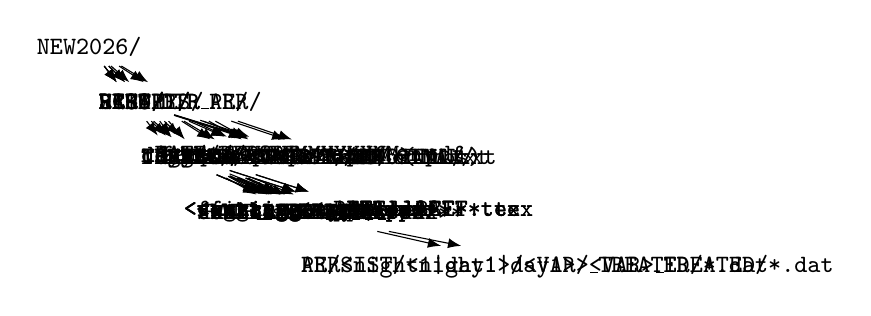
\begin{tikzpicture}[
  font=\ttfamily\small,
  grow=down,
  level distance=7mm,
  sibling distance=0mm,
  edge from parent/.style={-Latex, draw},
  every node/.style={anchor=west},
  folder/.style={},
  desc/.style={font=\rmfamily\small\itshape, anchor=west}
]

% Root
\node[folder] (root) {NEW2026/}
  child { node[folder] (scripts) {SCRIPTS/}
    child { node[folder] {runall} }
    child { node[folder] {run\_<var>.sh} }
    child { node[folder] {run\_skills.sh} }
    child { node[folder] {compile\_report.sh} }
    child { node[folder] {fate-report-astro.env} }
  }
  child { node[folder] (prog) {PROG/}
    child { node[folder] {TEST\_AR/AR\_10min/ORIGINAL/} }
    child { node[folder] {TEST\_AR/PERSIST/ORIGINAL/} }
    child { node[folder] {NUMREC/ \& LIBPERSO/ (libs)} }
  }
  child { node[folder] (data) {DATA/}
    child { node[folder] {TREATED/}
      child { node[folder] {FATE\_10min\_AR/}
        child { node[folder] {AR/<night1|day1>/<VAR>\_TREATED/*.dat} }
        child { node[folder] {PERSIST/<night1|day1>/<VAR>\_TREATED/*.dat} }
      }
    }
  }
  child { node[folder] (listsar) {LIST\_DIR\_AR/}
    child { node[folder] {list\_<VAR>.txt} }
    child { node[folder] {list\_<VAR>\_LastMonth.txt} }
  }
  child { node[folder] (listsper) {LIST\_DIR\_PER/}
    child { node[folder] {list\_<VAR>.txt} }
    child { node[folder] {list\_<VAR>\_LastMonth.txt} }
  }
  child { node[folder] (wrk) {WRKDIR/}
    child { node[folder] {night1/}
      child { node[folder] {skills\_BEFAFT\_<var>*} }
      child { node[folder] {skills\_PER\_<var>*} }
      child { node[folder] {figures\_<var>.tex} }
      child { node[folder] {contingency\_tableBEF*.tex} }
      child { node[folder] {contingency\_tableAFT*.tex} }
      child { node[folder] {tablePODs*.tex} }
      child { node[folder] {table\_skills\_*.tex} }
    }
    child { node[folder] {day1/}
      child { node[folder] {skills\_BEFAFT\_<var>*} }
      child { node[folder] {skills\_PER\_<var>*} }
      child { node[folder] {figures\_<var>.tex} }
      child { node[folder] {contingency\_tableBEF*.tex} }
      child { node[folder] {contingency\_tableAFT*.tex} }
      child { node[folder] {tablePODs*.tex} }
      child { node[folder] {table\_skills\_*.tex} }
    }
  }
  child { node[folder] (figs) {FIGS/}
    child { node[folder] {night1/}
      child { node[folder] {<var>\_... \_BEF.pdf} }
      child { node[folder] {<var>\_... \_AFT.pdf} }
      child { node[folder] {<var>\_... \_per.pdf} }
    }
    child { node[folder] {day1/}
      child { node[folder] {<var>\_... \_BEF.pdf} }
      child { node[folder] {<var>\_... \_AFT.pdf} }
      child { node[folder] {<var>\_... \_per.pdf} }
    }
  }
  child { node[folder] (report) {REPORT/}
    child { node[folder] {FATE-REPORT\_<YYYYMM>.pdf} }
    child { node[folder] {Annex\_<YYYYMM>.pdf} }
  };

\end{tikzpicture}
\caption{Filesystem-tree style view of the runtime directory structure and expected artifacts.}
\label{fig:filesystem-tree}
\end{figure}

\noindent\textbf{Interpretation notes:}
\begin{itemize}
  \item \texttt{LIST\_DIR\_AR} and \texttt{LIST\_DIR\_PER} contain the controlling lists of dates/files; \texttt{runall} creates symlinks to these for the current run.
  \item \texttt{WRKDIR/<block>} contains the primary intermediate products: skill logs and LaTeX fragments.
  \item \texttt{FIGS/<block>} contains the PDF figures referenced by \texttt{figures\_<var>.tex}.
  \item \texttt{REPORT/} contains only the final deliverables (PDFs) after \texttt{compile\_report.sh}.
\end{itemize}

\end{figure}


\subsection*{1. Entry Point}

\begin{itemize}
    \item \texttt{runall} is executed
    \item It automatically loads: \texttt{\$HOME/NEW2026/SCRIPTS/fate-report-astro.env}
\end{itemize}

\subsection*{2. Environment Loading}

The environment file \texttt{\$HOME/NEW2026/SCRIPTS/fate-report-astro.env} defines:

\begin{itemize}
    \item Data directories
    \item Working directory
    \item Forecast configuration
    \item Compilation paths
    \item Date ranges
    \item Report template paths
\end{itemize}

\subsection*{3. Housekeeping}

\begin{itemize}
    \item Clean \texttt{WRKDIR}
    \item Remove previous .tex, .log, .aux, .png, skills files
    \item Create subdirectories: \texttt{night1}, \texttt{day1}
\end{itemize}

\subsection*{4. Variable Loop}

For each forecast block (e.g. NIGHT1, DAY1):

\begin{itemize}
    \item Set \texttt{fcst\_target} and \texttt{fcst\_length}
    \item Loop over variables: RH, WS, WD, PWV, SEE, TAU, GLF
    \item Execute \texttt{run\_<var>.sh}
    \item Execute \texttt{run\_skills.sh}
\end{itemize}

\subsection*{5. Inside run\_$<$var$>$.sh}

\begin{enumerate}
    \item Source environment and \texttt{functions.sh}
    \item Retrieve variable attributes via \texttt{get\_var\_attr()}
    \item Define working directory: \texttt{WRKDIR/\{FCST\_DAY\}\{FCST\_LEN\}}
    \item Compile Fortran program via \texttt{gfortran}
    \item Run executable with heredoc input parameters
    \item Produce:
        \begin{itemize}
            \item skills\_BEFAFT\_<prefix>
            \item skills\_PER\_<prefix>
            \item PDF figures
        \end{itemize}
    \item Parse skills files using grep/awk
    \item Generate LaTeX fragments and tables:
        \begin{itemize}
            \item contingency\_tableBEF*.tex
            \item contingency\_tableAFT*.tex
            \item tablePODs*.tex
            \item figures\_$<$prefix$>$.tex
        \end{itemize}
\end{enumerate}

\subsection*{6. compile\_report.sh}

\begin{itemize}
    \item Concatenate generated .tex fragments
    \item Insert static sections (Introduction, References, Logs)
    \item Compile LaTeX into final PDF
    \item Output to \texttt{REPORTDIR}
\end{itemize}

\section{fate-report-astro.env Configuration}

\subsection{Forecast Type}

\textbf{FCST\_TYPE}

\begin{itemize}
    \item Allowed: \texttt{10min} or \texttt{mean}
    \item Determines DATA\_ROOT\_DIR and DATA\_PERS\_DIR
\end{itemize}

\subsection{Scientific Parameters}

\begin{longtable}{|p{4cm}|p{9cm}|}
\hline
GG & Scenario identifier passed to Fortran \\ \hline
HH & Time resolution identifier (e.g. 1H) \\ \hline
STARTMINUTE & Start minute for statistics window \\ \hline
ENDMINUTE & End minute for statistics window \\ \hline
LIMIT & Threshold parameter passed to Fortran \\ \hline
TAIL & File extension (typically .dat) \\ \hline
\end{longtable}

\subsection{Directories}

\begin{longtable}{|p{4cm}|p{9cm}|}
\hline
PROG\_ROOT\_DIR & Location of AR Fortran programs \\ \hline
PERS\_ROOT\_DIR & Location of Persistence Fortran programs \\ \hline
LIBPERSO\_DIR & Custom library path for compilation \\ \hline
NUMREC\_DIR & Numerical Recipes library path \\ \hline
WRKDIR & Working directory for intermediate files \\ \hline
FIGS\_ROOT\_DIR & Output directory for figures \\ \hline
REPORTDIR & Final PDF output directory \\ \hline
\end{longtable}

\subsection{Date Configuration}

Defines report period and affects captions and filenames:

\begin{itemize}
    \item STARTOFSERVICE\_YYYY/MM/DD
    \item ENDOFSERVICE\_YYYY/MM/DD
    \item Automatically derived date strings
\end{itemize}

\section{Critical Operational Parameters}

Before running \texttt{runall}, verify:

\begin{enumerate}
    \item FCST\_TYPE consistency with data directories
    \item PROG\_ROOT\_DIR contains required .f90 files
    \item Libraries compile correctly
    \item LIST\_* files exist and are coherent with the dates you want\footnote{\textbf{This step is crucial}}
    \item WRKDIR and REPORTDIR have write permissions
\end{enumerate}

\section{Operational Summary}

\begin{enumerate}
    \item Configure fate-report-astro.env
    \item Ensure data and list files are correct
    \item Execute: \texttt{./runall}
    \item Review output in WRKDIR and REPORTDIR
\end{enumerate}



\newpage
\section{Production-Ready Operational Checklist}

This checklist is intended for operational use before executing 
\texttt{SCRIPTS/runall} in a production environment.

\subsection{1. Environment Configuration Validation}

\begin{itemize}
    \item [ ] Verify \texttt{FCST\_TYPE} is correct (10min or mean).
    \item [ ] Confirm \texttt{STARTMINUTE} and \texttt{ENDMINUTE} match operational window.
    \item [ ] Confirm \texttt{GG} and \texttt{HH} are consistent with data resolution.
    \item [ ] Validate service date range:
        \begin{itemize}
            \item [ ] \texttt{STARTOFSERVICE\_YYYY/MM/DD}
            \item [ ] \texttt{ENDOFSERVICE\_YYYY/MM/DD}
        \end{itemize}
\end{itemize}

\subsection{2. Directory Integrity}

\begin{itemize}
    \item [ ] \texttt{PROG\_ROOT\_DIR} exists and contains required \texttt{.f90} files.
    \item [ ] \texttt{PERS\_ROOT\_DIR} exists and contains persistence programs.
    \item [ ] \texttt{LIBPERSO\_DIR} and \texttt{NUMREC\_DIR} exist and are accessible.
    \item [ ] \texttt{DATA\_ROOT\_DIR} exists for selected FCST\_TYPE.
    \item [ ] \texttt{DATA\_PERS\_DIR} exists for selected FCST\_TYPE.
    \item [ ] \texttt{WRKDIR} exists and is writable.
    \item [ ] \texttt{FIGS\_ROOT\_DIR} exists and is writable.
    \item [ ] \texttt{REPORTDIR} exists and is writable.
\end{itemize}

\subsection{3. List File Consistency}

\begin{itemize}
    \item [ ] AR list files exist in \texttt{\$PROG\_ROOT\_DIR}.
    \item [ ] PERSISTENCE list files exist in \texttt{\$PERS\_ROOT\_DIR}.
    \item [ ] Symlinked \texttt{list\_<VAR>.txt} matches current reporting month.
    \item [ ] Number of nights (wc -l) consistent with expected sample size.
\end{itemize}

\subsection{4. Compilation Validation}

\begin{itemize}
    \item [ ] \texttt{gfortran} available in PATH.
    \item [ ] Test compile of one Fortran program successful.
    \item [ ] Linked libraries resolve correctly (no missing symbols).
\end{itemize}

\subsection{5. Runtime Dry-Run Test}

\begin{itemize}
    \item [ ] Execute one variable only (e.g. RH night1).
    \item [ ] Verify generation of:
        \begin{itemize}
            \item [ ] skills\_BEFAFT file
            \item [ ] skills\_PER file
            \item [ ] PDF figures
            \item [ ] LaTeX fragments
        \end{itemize}
    \item [ ] Check parsing of contingency tables (no empty values).
\end{itemize}

\subsection{6. Full Pipeline Execution}

\begin{itemize}
    \item [ ] Execute \texttt{./runall}
    \item [ ] Monitor for compilation errors.
    \item [ ] Confirm no missing skills files.
    \item [ ] Confirm all expected .tex fragments created.
\end{itemize}

\subsection{7. Report Validation}

\begin{itemize}
    \item [ ] Final PDF generated in \texttt{REPORTDIR}.
    \item [ ] Figures correctly embedded.
    \item [ ] Contingency tables populated.
    \item [ ] POD tables consistent with skills files.
    \item [ ] Date strings correct in captions.
\end{itemize}

\subsection{8. Post-Run Archiving}

\begin{itemize}
    \item [ ] Archive generated list files.
    \item [ ] Archive environment file used for this run.
    \item [ ] Tag report version (e.g. YYYYMM).
\end{itemize}

\subsection{Production Readiness Gate}

The run can be considered production-valid only if:

\begin{itemize}
    \item No compilation errors occurred.
    \item No missing skills files were detected.
    \item All tables contain non-empty numerical values.
    \item The final PDF passes visual validation.
\end{itemize}

\clearpage
\section{Directory Structure (Filesystem Representation)}

The operational directory structure is reported below using a filesystem-style
representation. Each block includes a short description of its purpose.

\subsection*{Filesystem Tree}

\begin{verbatim}
NEW2026/
|
|---- SCRIPTS/
|   |---- runall                     # Main orchestration script
|   |---- run_<var>.sh               # Variable-specific execution scripts
|   |---- run_skills.sh              # Skill aggregation
|   |---- compile_report.sh          # LaTeX compilation and report assembly
|   `---- fate-report-astro.env      # Environment configuration
|
|---- PROG/
|   |---- TEST_AR/
|   |   |---- AR_10min/ORIGINAL/     # Fortran AR codes (.f90)
|   |   `---- PERSIST/ORIGINAL/      # Fortran persistence codes (.f90)
|   |---- NUMREC/                    # Numerical Recipes library
|   `---- LIBPERSO/                  # Custom compiled libraries
|
|---- DATA/
|   `---- TREATED/
|       `---- FATE_10min_AR/
|           |---- AR/
|           |   |---- night1/<VAR>_TREATED/*.dat
|           |   `---- day1/<VAR>_TREATED/*.dat
|           `---- PERSIST/
|               |---- night1/<VAR>_TREATED/*.dat
|               `---- day1/<VAR>_TREATED/*.dat
|
|---- LIST_DIR_AR/
|   |---- list_<VAR>.txt
|   `---- list_<VAR>_LastMonth.txt
|
|---- LIST_DIR_PER/
|   |---- list_<VAR>.txt
|   `---- list_<VAR>_LastMonth.txt
|
|---- WRKDIR/
|   |---- night1/
|   |   |---- skills_BEFAFT_<var>*
|   |   |---- skills_PER_<var>*
|   |   |---- contingency_table*.tex
|   |   |---- tablePODs*.tex
|   |   |---- table_skills_*.tex
|   |   `---- figures_<var>.tex
|   |
|   `---- day1/
|       |---- skills_BEFAFT_<var>*
|       |---- skills_PER_<var>*
|       |---- contingency_table*.tex
|       |---- tablePODs*.tex
|       |---- table_skills_*.tex
|       `---- figures_<var>.tex
|
|---- FIGS/
|   |---- night1/
|   |   |---- <var>_..._BEF.pdf
|   |   |---- <var>_..._AFT.pdf
|   |   `---- <var>_..._per.pdf
|   |
|   `---- day1/
|       |---- <var>_..._BEF.pdf
|       |---- <var>_..._AFT.pdf
|       `---- <var>_..._per.pdf
|
`---- REPORT/
    |---- FATE-REPORT_<YYYYMM>.pdf
    `---- Annex_<YYYYMM>.pdf
\end{verbatim}

\subsection*{Interpretation}

\begin{itemize}
    \item \textbf{SCRIPTS/} contains orchestration logic and configuration.
    \item \textbf{PROG/} contains Fortran scientific computation codes and libraries.
    \item \textbf{DATA/} contains treated AR and Persistence datasets.
    \item \textbf{LIST\_DIR\_AR / LIST\_DIR\_PER} control which nights/files are processed.
    \item \textbf{WRKDIR/} contains intermediate products (skills files and LaTeX fragments).
    \item \textbf{FIGS/} contains generated PDF figures for each variable and block.
    \item \textbf{REPORT/} contains final production-ready PDF reports.
\end{itemize}

\end{document}